% bce_imbalance.tex
% Triedna nevyváženosť: podiel pozitívnych hrán ρ+ = 2/(n-1) pre rôzne n
% Použitie: \resizebox{0.65\textwidth}{!}{% bce_imbalance.tex
% Triedna nevyváženosť: podiel pozitívnych hrán ρ+ = 2/(n-1) pre rôzne n
% Použitie: \resizebox{0.65\textwidth}{!}{% bce_imbalance.tex
% Triedna nevyváženosť: podiel pozitívnych hrán ρ+ = 2/(n-1) pre rôzne n
% Použitie: \resizebox{0.65\textwidth}{!}{% bce_imbalance.tex
% Triedna nevyváženosť: podiel pozitívnych hrán ρ+ = 2/(n-1) pre rôzne n
% Použitie: \resizebox{0.65\textwidth}{!}{\input{figures/tikz/bce_imbalance}}
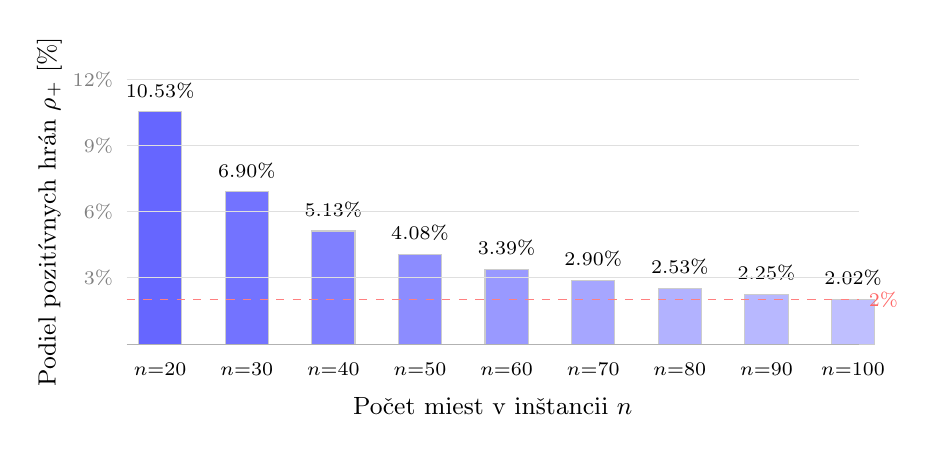
\begin{tikzpicture}[
    font=\small
]

%% Hodnoty ρ+ = 2/(n-1) v percentách pre n = 20,30,40,50,60,70,80,90,100
%% n=20: 10.53%, n=30: 6.90%, n=40: 5.13%, n=50: 4.08%
%% n=60: 3.39%, n=70: 2.90%, n=80: 2.53%, n=90: 2.25%, n=100: 2.02%

\def\barwidth{0.55}
\def\xscale{1.10}   % vzdialenosť medzi stĺpcami
\def\yscale{3.0}    % výška 1% = koľko cm

%% Pomocné premenné: (n, rho%, label_y_offset)
\foreach \idx/\n/\rho/\col in {
    1/20/10.53/blue!60,
    2/30/6.90/blue!55,
    3/40/5.13/blue!50,
    4/50/4.08/blue!45,
    5/60/3.39/blue!40,
    6/70/2.90/blue!35,
    7/80/2.53/blue!30,
    8/90/2.25/blue!28,
    9/100/2.02/blue!25
} {
    \pgfmathsetmacro\xpos{(\idx-1)*\xscale}
    \pgfmathsetmacro\barh{\rho * 0.28}  % scale: 10.53% → ~2.95 cm

    %% Stĺpec
    \fill[\col] (\xpos, 0) rectangle ++(\barwidth, \barh);
    \draw[gray!40, thin] (\xpos, 0) rectangle ++(\barwidth, \barh);

    %% Hodnota nad stĺpcom
    \node[font=\scriptsize, anchor=south] at (\xpos + \barwidth/2, \barh + 0.05)
        {\rho\%};

    %% Popis osi X
    \node[font=\scriptsize, anchor=north] at (\xpos + \barwidth/2, -0.12)
        {\(n{=}\n\)};
}

%% Os X
\draw[gray!60, -] (-0.15, 0) -- (9.15, 0);

%% Os Y s mriežkou
\foreach \yval/\ypct in {0.84/3, 1.68/6, 2.52/9, 3.36/12} {
    \draw[gray!25, thin] (-0.15, \yval) -- (9.15, \yval);
    \node[font=\scriptsize, anchor=east, gray] at (-0.2, \yval) {\ypct\%};
}

%% Popis osí
\node[font=\small, anchor=north] at (4.5, -0.55)
    {Počet miest v inštancii \(n\)};
\node[font=\small, rotate=90, anchor=south] at (-0.85, 1.68)
    {Podiel pozitívnych hrán \(\rho_+\) [\%]};

%% Zvýraznenie hranice 2% — horizontálna prerušovaná čiara
\draw[red!50, dashed, thin] (-0.15, 0.566) -- (9.15, 0.566)
    node[right, font=\scriptsize, red!60] {2\%};

\end{tikzpicture}
}
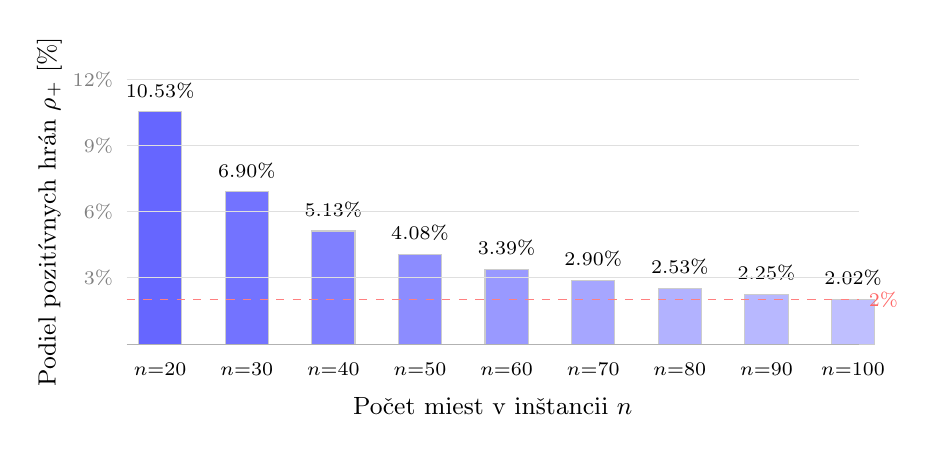
\begin{tikzpicture}[
    font=\small
]

%% Hodnoty ρ+ = 2/(n-1) v percentách pre n = 20,30,40,50,60,70,80,90,100
%% n=20: 10.53%, n=30: 6.90%, n=40: 5.13%, n=50: 4.08%
%% n=60: 3.39%, n=70: 2.90%, n=80: 2.53%, n=90: 2.25%, n=100: 2.02%

\def\barwidth{0.55}
\def\xscale{1.10}   % vzdialenosť medzi stĺpcami
\def\yscale{3.0}    % výška 1% = koľko cm

%% Pomocné premenné: (n, rho%, label_y_offset)
\foreach \idx/\n/\rho/\col in {
    1/20/10.53/blue!60,
    2/30/6.90/blue!55,
    3/40/5.13/blue!50,
    4/50/4.08/blue!45,
    5/60/3.39/blue!40,
    6/70/2.90/blue!35,
    7/80/2.53/blue!30,
    8/90/2.25/blue!28,
    9/100/2.02/blue!25
} {
    \pgfmathsetmacro\xpos{(\idx-1)*\xscale}
    \pgfmathsetmacro\barh{\rho * 0.28}  % scale: 10.53% → ~2.95 cm

    %% Stĺpec
    \fill[\col] (\xpos, 0) rectangle ++(\barwidth, \barh);
    \draw[gray!40, thin] (\xpos, 0) rectangle ++(\barwidth, \barh);

    %% Hodnota nad stĺpcom
    \node[font=\scriptsize, anchor=south] at (\xpos + \barwidth/2, \barh + 0.05)
        {\rho\%};

    %% Popis osi X
    \node[font=\scriptsize, anchor=north] at (\xpos + \barwidth/2, -0.12)
        {\(n{=}\n\)};
}

%% Os X
\draw[gray!60, -] (-0.15, 0) -- (9.15, 0);

%% Os Y s mriežkou
\foreach \yval/\ypct in {0.84/3, 1.68/6, 2.52/9, 3.36/12} {
    \draw[gray!25, thin] (-0.15, \yval) -- (9.15, \yval);
    \node[font=\scriptsize, anchor=east, gray] at (-0.2, \yval) {\ypct\%};
}

%% Popis osí
\node[font=\small, anchor=north] at (4.5, -0.55)
    {Počet miest v inštancii \(n\)};
\node[font=\small, rotate=90, anchor=south] at (-0.85, 1.68)
    {Podiel pozitívnych hrán \(\rho_+\) [\%]};

%% Zvýraznenie hranice 2% — horizontálna prerušovaná čiara
\draw[red!50, dashed, thin] (-0.15, 0.566) -- (9.15, 0.566)
    node[right, font=\scriptsize, red!60] {2\%};

\end{tikzpicture}
}
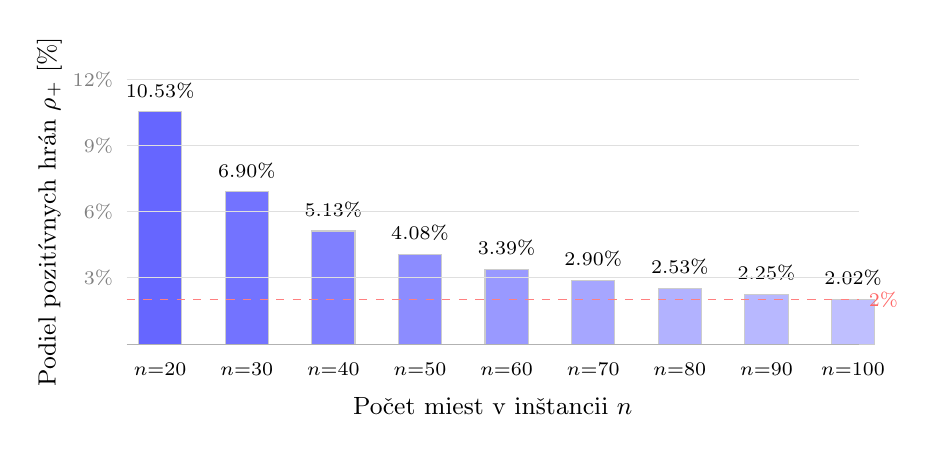
\begin{tikzpicture}[
    font=\small
]

%% Hodnoty ρ+ = 2/(n-1) v percentách pre n = 20,30,40,50,60,70,80,90,100
%% n=20: 10.53%, n=30: 6.90%, n=40: 5.13%, n=50: 4.08%
%% n=60: 3.39%, n=70: 2.90%, n=80: 2.53%, n=90: 2.25%, n=100: 2.02%

\def\barwidth{0.55}
\def\xscale{1.10}   % vzdialenosť medzi stĺpcami
\def\yscale{3.0}    % výška 1% = koľko cm

%% Pomocné premenné: (n, rho%, label_y_offset)
\foreach \idx/\n/\rho/\col in {
    1/20/10.53/blue!60,
    2/30/6.90/blue!55,
    3/40/5.13/blue!50,
    4/50/4.08/blue!45,
    5/60/3.39/blue!40,
    6/70/2.90/blue!35,
    7/80/2.53/blue!30,
    8/90/2.25/blue!28,
    9/100/2.02/blue!25
} {
    \pgfmathsetmacro\xpos{(\idx-1)*\xscale}
    \pgfmathsetmacro\barh{\rho * 0.28}  % scale: 10.53% → ~2.95 cm

    %% Stĺpec
    \fill[\col] (\xpos, 0) rectangle ++(\barwidth, \barh);
    \draw[gray!40, thin] (\xpos, 0) rectangle ++(\barwidth, \barh);

    %% Hodnota nad stĺpcom
    \node[font=\scriptsize, anchor=south] at (\xpos + \barwidth/2, \barh + 0.05)
        {\rho\%};

    %% Popis osi X
    \node[font=\scriptsize, anchor=north] at (\xpos + \barwidth/2, -0.12)
        {\(n{=}\n\)};
}

%% Os X
\draw[gray!60, -] (-0.15, 0) -- (9.15, 0);

%% Os Y s mriežkou
\foreach \yval/\ypct in {0.84/3, 1.68/6, 2.52/9, 3.36/12} {
    \draw[gray!25, thin] (-0.15, \yval) -- (9.15, \yval);
    \node[font=\scriptsize, anchor=east, gray] at (-0.2, \yval) {\ypct\%};
}

%% Popis osí
\node[font=\small, anchor=north] at (4.5, -0.55)
    {Počet miest v inštancii \(n\)};
\node[font=\small, rotate=90, anchor=south] at (-0.85, 1.68)
    {Podiel pozitívnych hrán \(\rho_+\) [\%]};

%% Zvýraznenie hranice 2% — horizontálna prerušovaná čiara
\draw[red!50, dashed, thin] (-0.15, 0.566) -- (9.15, 0.566)
    node[right, font=\scriptsize, red!60] {2\%};

\end{tikzpicture}
}
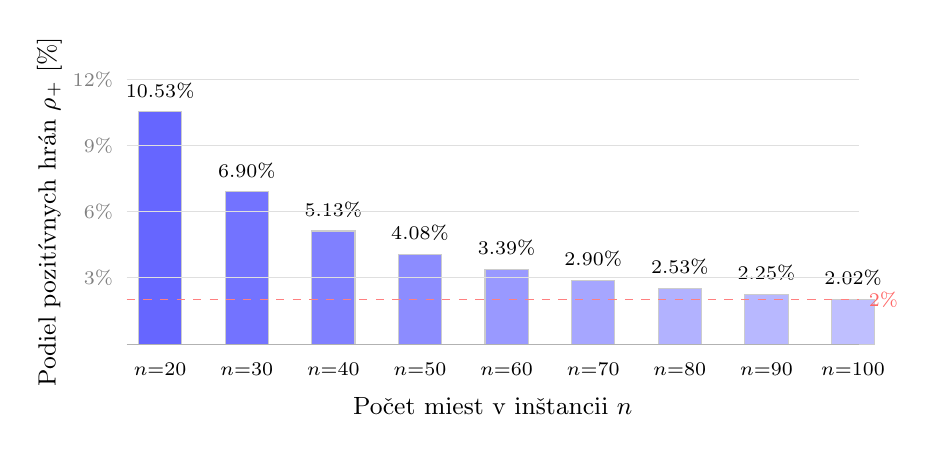
\begin{tikzpicture}[
    font=\small
]

%% Hodnoty ρ+ = 2/(n-1) v percentách pre n = 20,30,40,50,60,70,80,90,100
%% n=20: 10.53%, n=30: 6.90%, n=40: 5.13%, n=50: 4.08%
%% n=60: 3.39%, n=70: 2.90%, n=80: 2.53%, n=90: 2.25%, n=100: 2.02%

\def\barwidth{0.55}
\def\xscale{1.10}   % vzdialenosť medzi stĺpcami
\def\yscale{3.0}    % výška 1% = koľko cm

%% Pomocné premenné: (n, rho%, label_y_offset)
\foreach \idx/\n/\rho/\col in {
    1/20/10.53/blue!60,
    2/30/6.90/blue!55,
    3/40/5.13/blue!50,
    4/50/4.08/blue!45,
    5/60/3.39/blue!40,
    6/70/2.90/blue!35,
    7/80/2.53/blue!30,
    8/90/2.25/blue!28,
    9/100/2.02/blue!25
} {
    \pgfmathsetmacro\xpos{(\idx-1)*\xscale}
    \pgfmathsetmacro\barh{\rho * 0.28}  % scale: 10.53% → ~2.95 cm

    %% Stĺpec
    \fill[\col] (\xpos, 0) rectangle ++(\barwidth, \barh);
    \draw[gray!40, thin] (\xpos, 0) rectangle ++(\barwidth, \barh);

    %% Hodnota nad stĺpcom
    \node[font=\scriptsize, anchor=south] at (\xpos + \barwidth/2, \barh + 0.05)
        {\rho\%};

    %% Popis osi X
    \node[font=\scriptsize, anchor=north] at (\xpos + \barwidth/2, -0.12)
        {\(n{=}\n\)};
}

%% Os X
\draw[gray!60, -] (-0.15, 0) -- (9.15, 0);

%% Os Y s mriežkou
\foreach \yval/\ypct in {0.84/3, 1.68/6, 2.52/9, 3.36/12} {
    \draw[gray!25, thin] (-0.15, \yval) -- (9.15, \yval);
    \node[font=\scriptsize, anchor=east, gray] at (-0.2, \yval) {\ypct\%};
}

%% Popis osí
\node[font=\small, anchor=north] at (4.5, -0.55)
    {Počet miest v inštancii \(n\)};
\node[font=\small, rotate=90, anchor=south] at (-0.85, 1.68)
    {Podiel pozitívnych hrán \(\rho_+\) [\%]};

%% Zvýraznenie hranice 2% — horizontálna prerušovaná čiara
\draw[red!50, dashed, thin] (-0.15, 0.566) -- (9.15, 0.566)
    node[right, font=\scriptsize, red!60] {2\%};

\end{tikzpicture}
